\section{Analiza funkcjonalna systemu}
\subsection{Diagram przypadków użycia}
\begin{figure}[h]
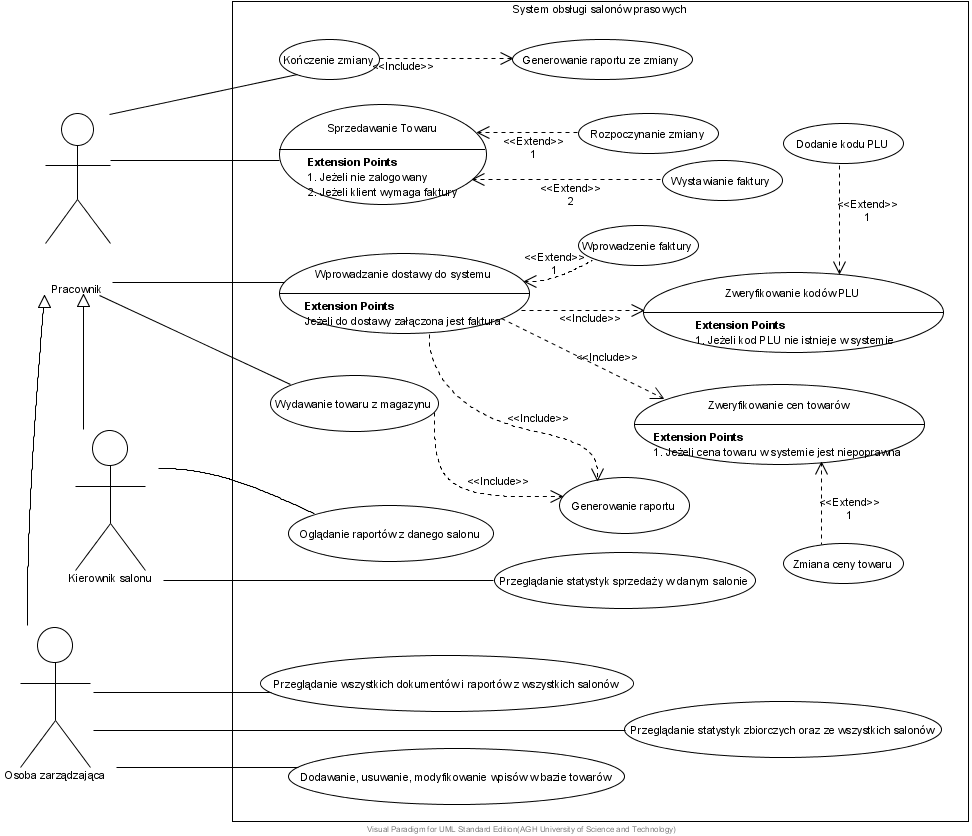
\includegraphics[width=1\textwidth]{gfx/usecase.png}
%TODO Wstawić diagram z UseCase
\caption{Diagram przypadków użycia systemu}
\end{figure}
\clearpage
\subsection{Diagram kontekstowy (przepływu danych - poziom 0)}
\begin{figure}[h]
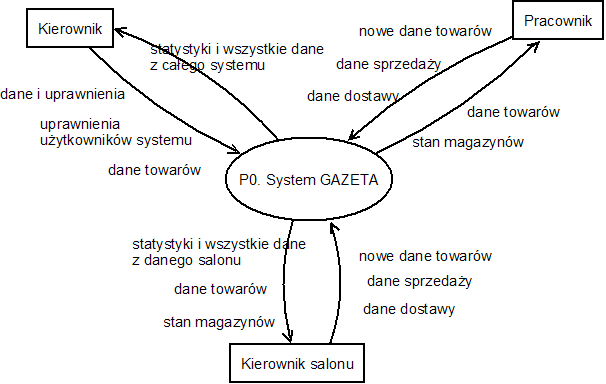
\includegraphics[width=1\textwidth]{gfx/dfd-0.png}
\caption{DFD - poziom 0 (diagram kontekstowy)}
\end{figure}
\clearpage
\subsection{Diagram przepływu danych - poziom 1}
\begin{figure}[h]
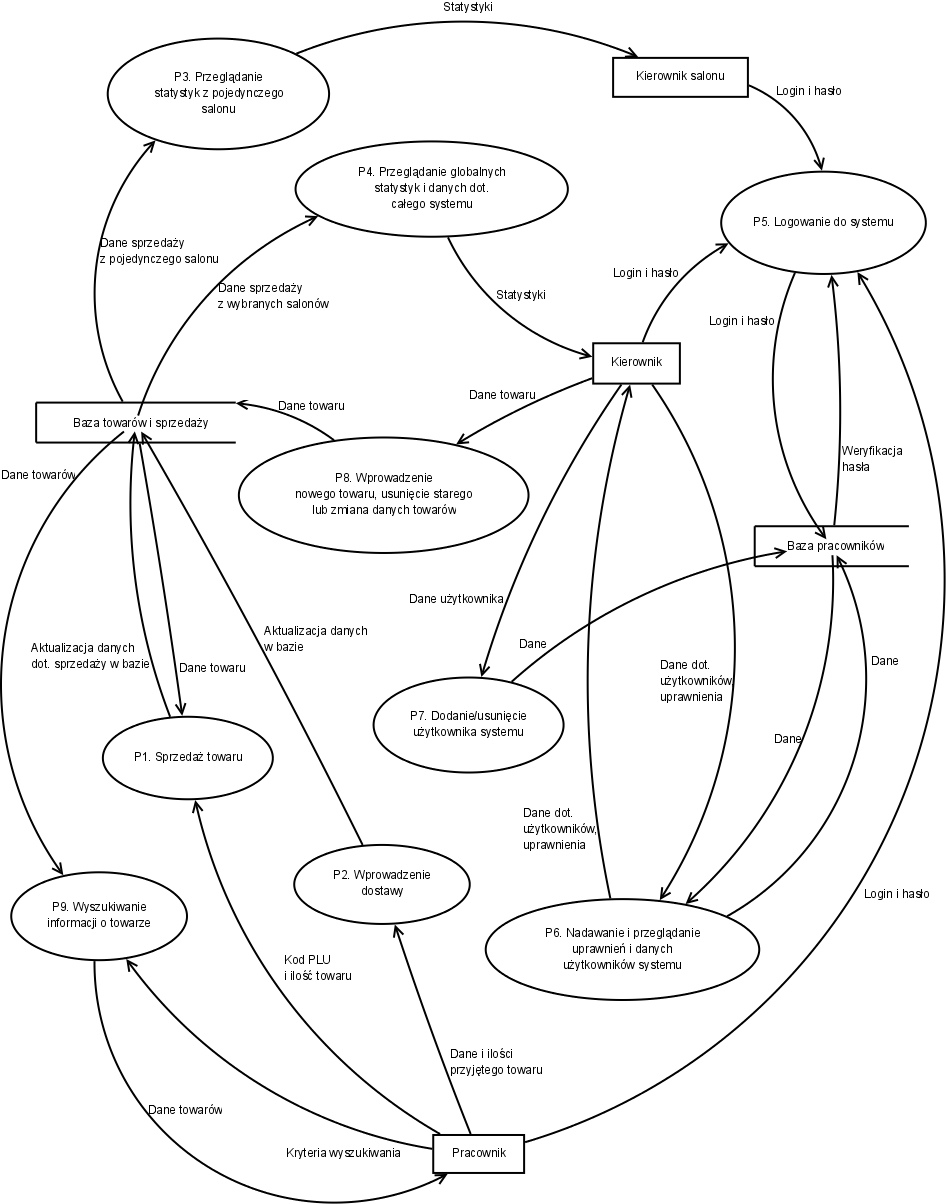
\includegraphics[width=1\textwidth]{gfx/dfd-1.png}
\caption{DFD - poziom 1}
\end{figure}
\clearpage
\subsection{Diagramy przepływu danych - poziom 2}
\subsubsection{Diagram przepływu danych - poziom 2.1}
\begin{figure}[h]
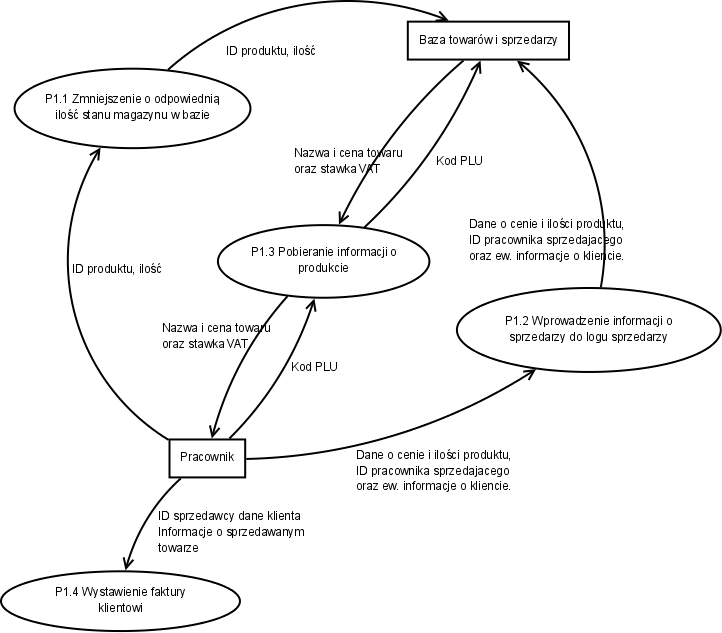
\includegraphics[width=1\textwidth]{gfx/dfd-2-1.png}
\caption{DFD - poziom 2.1}
\end{figure}
\clearpage
\subsubsection{Diagram przepływu danych - poziom 2.2}
\begin{figure}[h]
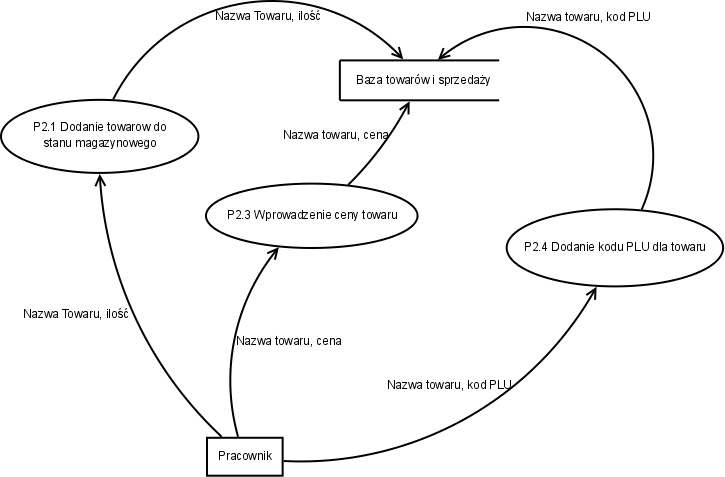
\includegraphics[width=1\textwidth]{gfx/dfd-2-2.png}
\caption{DFD - poziom 2.2}
\end{figure}
\clearpage
\subsubsection{Diagram przepływu danych - poziom 2.3}
\begin{figure}[h]
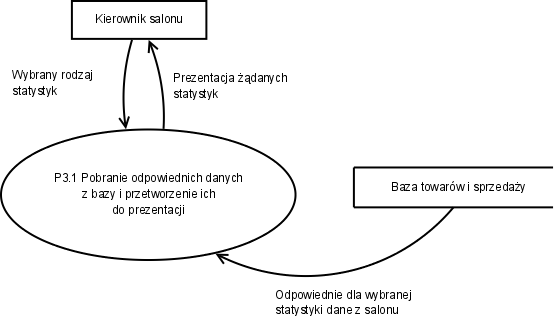
\includegraphics[width=1\textwidth]{gfx/dfd-2-3.png}
\caption{DFD - poziom 2.3}
\end{figure}
\clearpage
\subsubsection{Diagram przepływu danych - poziom 2.4}
\begin{figure}[h]
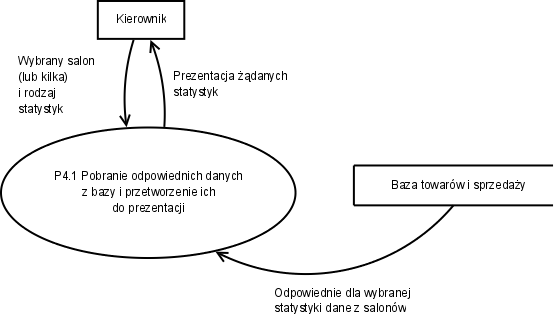
\includegraphics[width=1\textwidth]{gfx/dfd-2-4.png}
\caption{DFD - poziom 2.4}
\end{figure}
\clearpage
\subsubsection{Diagram przepływu danych - poziom 2.5}
\begin{figure}[h]
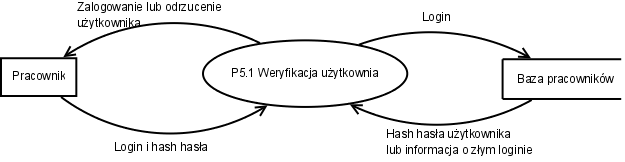
\includegraphics[width=1\textwidth]{gfx/dfd-2-5.png}
\caption{DFD - poziom 2.5}
\end{figure}
\clearpage
